\chapter{Marco Teórico}
    \begin{section}{Presentación}
        Las infracciones a las políticas de seguridad y los ataques han concentrado la atención sobre las capacidades de detección, investigación y mitigación de incidentes de seguridad de la información en  las organizaciones. Si bien no siempre es posible evitar un incidente de seguridad, es necesario detectar y responder rápidamente para minimizar el daño. Para ello, es preciso realizar inversiones inteligentes basadas en un plan de seguridad que comprenda la realidad y necesidades específicas de la organización, ya que un gran monto de dinero o equipos adquiridos por si mismos no garantizan una mayor protección. \par
        Este plan debe incluir personal especializado, procedimientos e infraestructura  adaptados a la organización, con una gestión de objetivos a cumplir a corto, mediano y largo plazo. \par
        Para las organizaciones que no cuentan con una capacidad de manejo de incidentes, la creación desde cero de un Computer Security Incident Response Team (CSIRT) puede ser un proceso complejo y costoso. Sin embargo, no es necesario una gran inversión para obtener las capacidades elementales ofrecidas por un CSIRT, ya que es posible desarrollar una solución específica y a escala de la organización. \par
        Una vez identificadas las necesidades de la organización, el proceso de creación del CSIRT requiere de la creación, colaboración y comunicación entre los tres pilares que lo componen: el personal, la tecnología y los procesos, como se muestra en la Figura \ref{fig:pilares}. \par
        \begin{figure}[H]
            \centering
            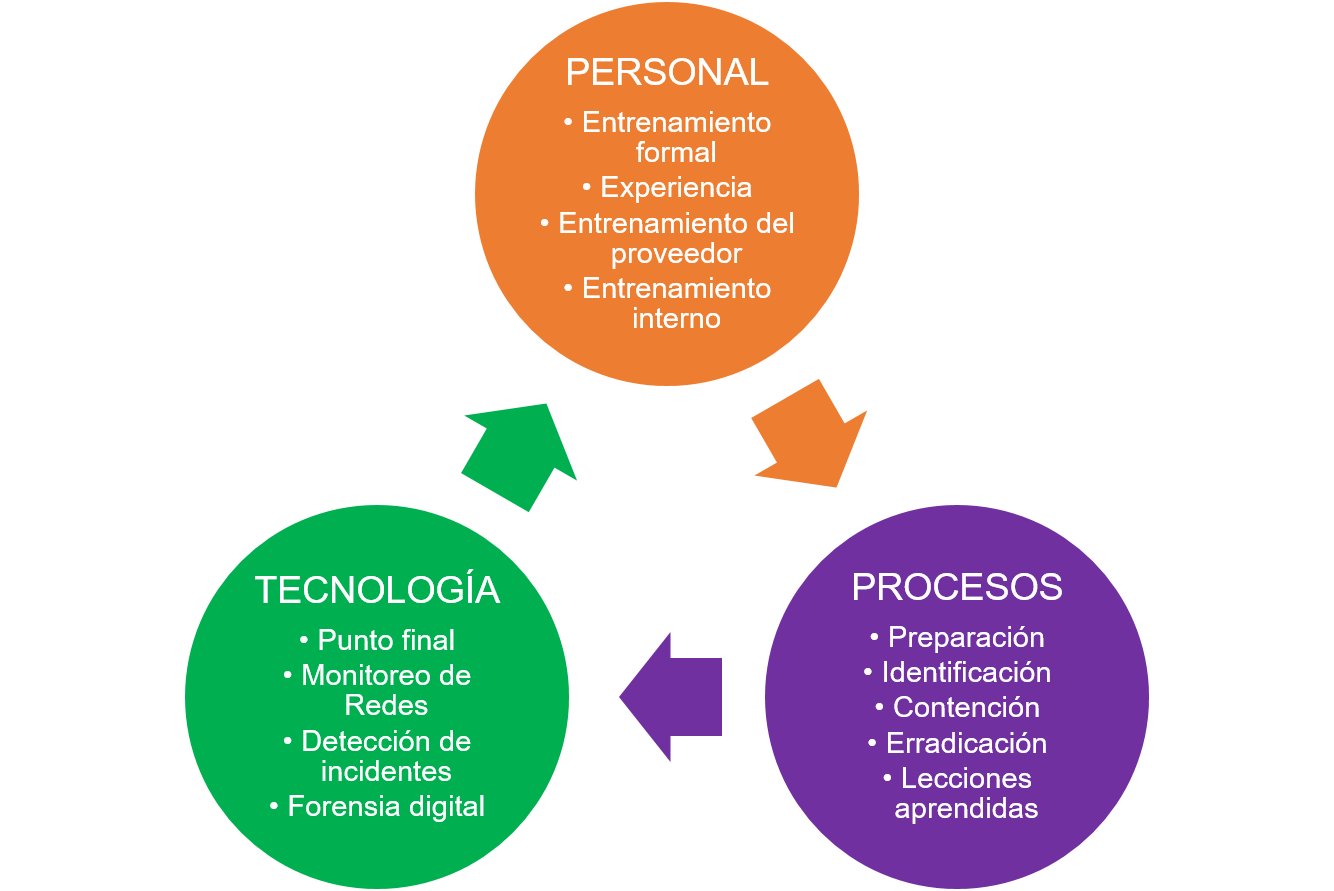
\includegraphics[width=1\textwidth]{./marco_teorico_imagenes/figura_1_pilares.png}
            \caption{Pilares de un CSIRT}
            \label{fig:pilares}
        \end{figure}
        %\par
        El CSIRT debe tener una perspectiva flexible y escalable para mantener el ritmo de las tácticas de los adversarios, acompañando el crecimiento y evolución de la organización. \par
    \end{section}
    
   \begin{section}{Personal}  
   En cuanto al personal, estos comprenden tanto a los encargados de dar respuesta a los incidentes como a los analistas del CSIRT. Si bien la propia organización puede designar a sus integrantes para asumir estas funciones, existen otras alternativas como la tercerización mediante empresas especializadas que proveen el servicio de Managed Security Service Provider (MSSP) o contratar especialistas en respuesta a incidentes en el caso de una emergencia o un problema complejo. Otra vía consiste en la creación de equipos híbridos compuestos por personal perteneciente a la organización y especialistas externos. \par
    De acuerdo a una encuesta del SANS Institute del año 2014 \cite{sans_1}, el 61\% de las organizaciones relevadas manifestaron haber recurrido a personal de emergencia para cubrir incidentes críticos y el 58 \% tenía un equipo de respuesta propio. Por lo que las organizaciones no siempre cubren sus necesidades con miembros de su propio personal y en algunos casos las tareas recaen por completo en los servicios de terceros. Esto se debe a que, sin importar la estructura del equipo, el personal de un CSIRT debe contar con el entrenamiento necesario para tratar con los cambios en las amenazas a las que se enfrenta. En el Cuadro \ref{table:1} se muestran las responsabilidades y la formación requerida para cada uno de los integrantes de un CSIRT. \par
    
    \begin{table}%[ht]
    \centering
        \begin{tabular}{ | m{10em} | m{16em}| m{11em} | } 
            \hline
            Título profesional & Tarea & Entrenamiento requerido \\ 
            \hline
            Nivel 1 - Analista de alertas & Supervisa continuamente la cola de alertas, monitorea el estado de los sensores y los puntos finales, clasifica las alertas de seguridad y recopila los datos necesarios para iniciar el trabajo de Nivel 2. & Procedimientos de triage de alerta y detección de intrusos. Gestión de redes, información de seguridad y eventos. Capacitación en investigación basada en host. \\ 
            \hline
            Nivel 2 - Analista de respuesta a incidentes & Realiza un análisis profundo de incidentes al correlacionar datos de varias fuentes y determina si un sistema crítico o un conjunto de datos se ha visto afectado. Asesora sobre su remediación. & Análisis avanzado de forensia de redes y basado en host. Procedimientos de respuesta a incidentes, revisiones de registros, evaluación básica de malware e inteligencia de amenazas. \\ 
            \hline
            Nivel 3 - Especialista en la materia & Se trata de un conjunto de especialistas que cubren distintas áreas de un CSIRT. 
            Actúan como “cazadores” de amenazas, sin esperar que se intensifiquen los incidentes. Se encuentra estrechamente involucrado en el desarrollo, ajuste e implementación de análisis de detección de amenazas.
             & Entrenamiento avanzado en detección de anomalías. Entrenamiento específico en herramientas para la agregación y análisis de datos e inteligencia de amenazas. 
            Poseen un conocimiento profundo en áreas como redes, puntos finales, inteligencia de amenazas, forensia e ingeniería inversa de malware, así como la infraestructura de IT subyacente.
            \\ 
             \hline
            Director del CSIRT & Administra recursos para incluir personal, presupuesto, programación de turnos y estrategias para cumplir con los acuerdos de nivel de servicio. Se comunica con la gerencia y sirve como persona de contacto en el caso de incidentes críticos. Proporciona una dirección general para el CSIRT. & Gestión de proyectos, formación en gestión de respuesta a incidentes, habilidades generales de gestión de personas y comunicación institucional.  \\
            \hline %linea final de tabla
        \end{tabular}
        \caption{Integrantes de un CSIRT y sus funciones}
        \label{table:1}
    \end{table}
    
   \end{section}
   
   \begin{section}{Procesos}  
   
   \end{section}
   \begin{section}{Tecnología}  
        \begin{subsection}{Agregando contexto a los incidentes}
        La incorporación de inteligencia de amenazas y otras informaciones de contexto tales como activos e identidades, contribuye al proceso de investigación del analista de un CSIRT. En determinados casos, la información inicial que está asociada a una alerta puede ser muy limitada, por ejemplo la dirección IP del punto final sospechoso es insuficiente por sí sola para tomar una decisión. \par
        Para que los analistas puedan investigar un incidente, generalmente necesitan más información, por ejemplo los nombres del dueño y de dominio de la máquina, registros DHCP para mapear la IP con el host al momento del incidente, etc. Si el sistema de monitoreo incorpora información de identidad y de los activos de información, entre otros datos de contexto, le permitirá al analista ahorrar tiempo y esfuerzo para priorizar los incidentes y elaborar la respuesta más apropiada.\par

        \end{subsection}
        \begin{subsection}{Agregando contexto a los incidentes}
        \end{subsection}
        
        \begin{subsection}{Definición de conductas normales}
        \end{subsection}
        
        \begin{subsection}{Inteligencia de amenazas}
        \end{subsection}
        
        \begin{subsection}{Obstáculos para el manejo eficiente de incidentes del CSIRT}
        \end{subsection}
   \end{section}
      
   \begin{section}{Ámbitos de actuación de los CSIRT}
        \begin{subsection}{Estado de la ciberseguridad en Argentina} 
            \begin{subsubsection}{Demanda de ciberseguridad Argentina}
            \end{subsubsection}
        \end{subsection}
   \end{section}

    \begin{section}{SIEM: Definición y funciones}
    
    \end{section}
    \begin{section}{Soluciones disponibles}
    
    
        \begin{subsection}{Soluciones comerciales}
        
        \end{subsection}
        \begin{subsection}{Soluciones gratuitas y de código abierto}
        
        
            \begin{subsubsection}{AlienVault OSSIM}
            
            \end{subsubsection}
            \begin{subsubsection}{Graylog}
            
            \end{subsubsection}
            \begin{subsubsection}{Elastic Stack}
            
            \end{subsubsection}
            \begin{subsubsection}{Security Onion}
            
            \end{subsubsection}
            
        \end{subsection} 
    \end{section}
    \begin{section}{Corolario}
    
    \end{section}
            
            
            
            
